\documentclass[conference]{IEEEtran}

\usepackage{graphicx}

\begin{document}

% paper title
\title{On Supporting Molecular Visualization on Grid Resources using Visual
  Programming Environments}

% author information
\author{\authorblockN{Sriram Krishnan\authorrefmark{1}\authorrefmark{2},
    Guillaume Vareille\authorrefmark{3},
    Wesley Goodman\authorrefmark{1},
    Luca Clementi\authorrefmark{1},\\
    Jane Ren\authorrefmark{1},
    Sargis Dallakyan\authorrefmark{3},
    Wilfred Li\authorrefmark{1}\authorrefmark{2},
    Michel Sanner\authorrefmark{3} and
    Peter Arzberger\authorrefmark{1}}
  \authorblockA{\authorrefmark{1}National Biomedical Computation Resource\\
    CRBS, UC San Diego, 9500 Gilman Dr, La Jolla, CA 92093}
  \authorblockA{\authorrefmark{2}San Diego Supercomputer Center\\
    UC San Diego MC 0505, 9500 Gilman Dr, La Jolla, CA 92093}
  \authorblockA{\authorrefmark{3}The Molecular Graphics Lab\\
    The Scripps Research Institute, La Jolla, CA 92093
    }
  \authorblockA{sriram@sdsc.edu, vareille@scripps.edu, \{wgoodman,
      lclement, j2ren@ucsd.edu\},\\
      wilfred@sdsc.edu, sanner@scripps.edu, parzberger@ucsd.edu}
  }


% make the title area
\maketitle

\begin{abstract}

  The visual programming paradigm provided by tools such as AVS \cite{avs},
  OpenDX \cite{opendx}, SciRun \cite{scirun}, etc have been around for a
  couple decades. Recently, with the advent of the Web 2.0 paradigm and the
  concept of {\em mashups} \cite{web2.0}, there has been renewed interest
  in such types of environments. Over the past several years, we have
  developed one such tool called Vision \cite{viper}, which is a
  component-based, application-domain agnostic, cross-platform visual
  programming environment. Meanwhile, advances in distributed and Grid
  computing have opened up avenues for scientists to run large simulations
  on a scale that was impossible until recent times. In the past, visual
  programming tools were generally limited to running scientific
  experiments on user's individual workstations, and had limited capability
  to use distributed resources. With the proliferation of Web services,
  distributed resources are much more easy to access from any workstation
  that is connected to the Internet. In particular, we have developed the
  Opal toolkit, which provides a mechanism to wrap scientific applications
  running on Grid resources as Web services, thus providing the clients
  with a simple Web API to the back-end computational functionality. Opal
  encapsulates standard Grid security mechanisms, schedulers, and state
  management for jobs, and also provides a mechanism to describe
  command-line arguments that can be used to automatically generate
  user-interfaces \cite{opal}. In this paper, we describe our current work
  on enabling access to scientific applications running on Grid resources
  via Opal from the Vision environment. We present brief overviews of both
  Vision and Opal, and discuss a scientific workflow that has been
  implemented with the above tools. We discuss our experiences, and plans
  for future work.

\end{abstract}

\section{Introduction}

- Scientific workflows: Michel

% TODO: Add more context 

The visual-programming paradigm provided by tools such as the AVS
\cite{avs}, OpenDX \cite{opendx}, or SciRun \cite{scirun} has been around
for a couple of decades. Recently, there has recently been a renewed
interest in this type of user interface and numerous pipelining tools have
become available, including: PHENIX [ref], pipeline pilot [ref], mapero
[ref], Orange [ref], Elefant [ref], Kepler \cite{kepler}, Taverna
\cite{taverna} to name a few.

These software environments, allow a user to construct a computational
network by placing nodes performing a specific task onto a canvas and
connecting their output and input ports using pipes that specify the flow
of data through the network. The appeal of this type of interface is that
the user can interactively construct networks of computational nodes that
correspond to simple programs without having to write a single line of
code. It provides an effective way to hide syntax details and data
structures used to store data from the user who in general cares more about
the result of the computation rather than these implementation details. In
other words it empowers users with an unprecedented level of flexibility in
using computers without having to become a programmer.

While some of these tools are highly specific to a given application
domain, other try to be more generic programming environments. However,
most of these programs are what we call “application-centric” (i.e. they
constitute the development environment for a specific application) rather
than being a software component that will integrate and dovetail nicely
with other software components and that does not make assumptions about the
domain of application.

% TODO: Add Grid stuff

- Grid computing: Sriram

\section {Visual Programming Environments}

\subsection {The Vision Environment}

% - Design -- workflow representation and control: Michel

% - API -- how to write Vision nodes, introspection, etc: Michel

Over the past 8 years we have developed Vision \cite{viper}, a
component-based, application-domain agnostic, cross-platform visual
programming environment. Vision has been designed as an extension to the
Python programming language thus providing a fully fledged, high level,
object-oriented, interpretive language for the interactive manipulation of
data and/or modification of the application itself.

The Vision framework was designed to dynamically load libraries of
computational nodes providing specific functionality. Not only does this
approach reduce the footprint of Vision in memory, but it also avoids
cluttering the interface with nodes that a particular user might not be
interested in using. Each library can define its own data types, allowing
the validation of data passed to a node before the node will execute. A
data type definition includes a description of the visual representation of
ports receiving or sending this data type, thus providing visual clues to
the user while he create the data flow by connecting output ports to input
ports. Port can be declared as required or optional. A node can only run if
all required ports present valid data. Introspection tools allow the user
to inspect data on input ports and output ports in real time.

Vision network nodes are Python objects that provide input ports and output
ports. When a node is scheduled for execution, it will collect the data on
its input ports and pass it ot the node’s compute function. This function
typically imports Python code from some other Python package to operate on
the data and produce a result, which is then sent to the node’s output
port. This important design features makes Vision “just another” user
interface to functionality available to any program running a Python
interpreter thus promoting code re-use and inter-operability. Moreover,
since the node’s compute function is written in the Python programming
language it can be inspected and modified interactively by the user.  In
fact, a node can be designed interactively in Vision using the node editor.
All modifications made to a node or a network, are saved in the network
description file. This file contains Python code that will recreate the
network when executed. We made this choice in order to avoid having to
define a format for describing networks and also to have access to the full
power of a programming language for the definition of these networks.

Vision supports the concept of MacroNodes which appear as a simple node in
a network, but encapsulate a sub-network. MacroNodes can exist inside
Macronodes, thus allowing a hierarchical visual representation of algorithm
and facilitating code reuse within Vision.

While execution of a node is typically triggered by new data presented on
its ports, a node can also be triggered by events such as the completion of
another node’s execution. Vision’s execution model allows for the partial
execution of networks. When a parameter changes or new data is provided for
a given node, only the sub-graph of children nodes depending on this
parameter or dataset will re-compute.

An iterate node supports the implementation of “for loops” in Vision. This
node loops over any sequence of Python objects and triggers the sub-network
of its children nodes for each one of the objects in the sequence. Begin
and end of loop events allow the accumulation of data during a loop and the
execution of code after the completion of the loop. 

To date, several libraries of nodes are available as seen in Figure
\ref{fig:vision-overview}. The standard library comprises nodes exposing
Python keywords (print, eval, setattr and call methods), along with nodes
enabling the generation of simple input data such as floats, integers, and
strings. The 3-D Visualization library is based on the DejaVu component and
provides nodes to create 3-D geometries and display them. The SymServ
library implements a set of nodes defining geometric transformations such
as symmetries, translation, rotation, helical arrangements etc. that can be
combined to created streams of nested 3-D transformations. The MolKit
library is based on the MolKit package and provides nodes to read molecular
data files and manipulate molecules. The Imaging library currently exposes
a subset of the functionality available in the Python Image Library (PIL)
thus enabling the creation of image processing pipelines.

So far, Vision has essentially been used in an interactive way with most
computational nodes running locally (i.e. in the same process as the Python
interpreter running Vision). In this paper we describe the addition of
support for nodes running web services. 

% TODO: Need a more useful screenshot
\begin{figure}
\begin{center}
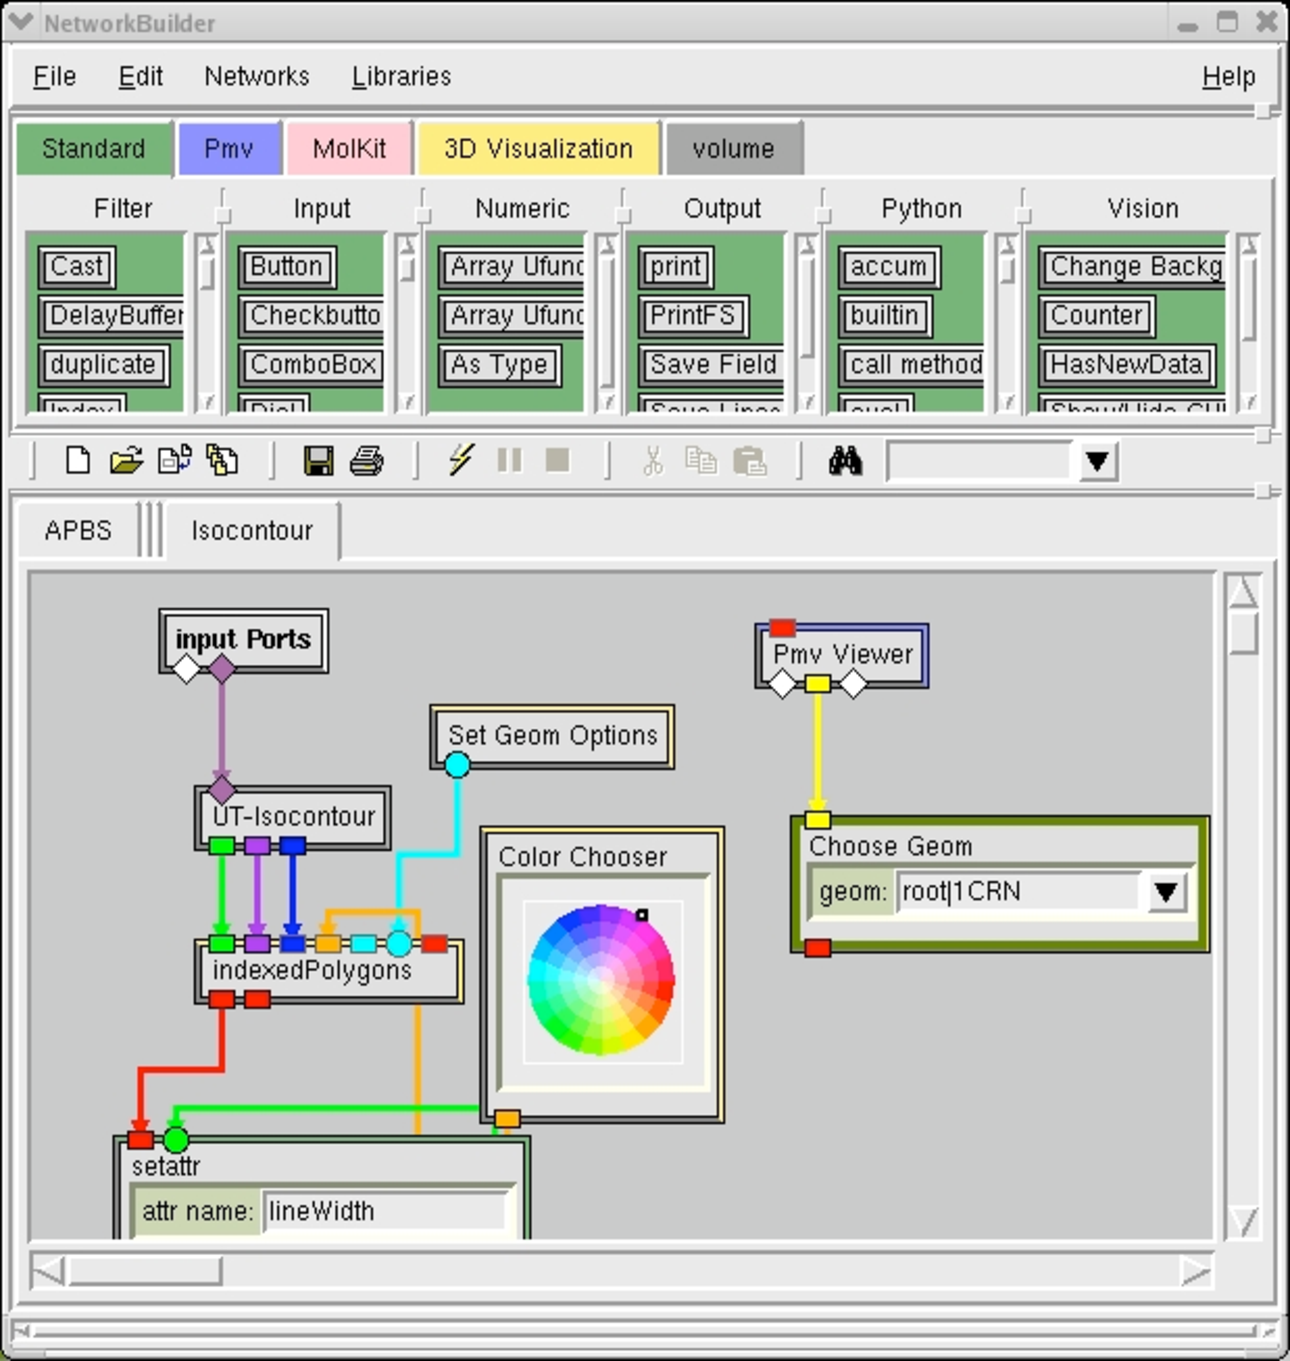
\includegraphics[width=8cm]{vision-overview}
\end{center}
\caption{A typical scientific workflow composed using the Vision interface}
\label{fig:vision-overview}
\end{figure}

\subsection {Related Work}

% - Comparison with other tools: Luca

%   - Kepler, Ptolemy and MoML

%   - Taverna, Scufl and Freeflou

Several tools have been developed by the scientific community to support
the design and execution of workflows. Each one of them use different
approaches to model a graphical environment for designing and executing
workflow. In this section we present three workflow management systems:
Kepler, Taverna, and AVS. This paragraph does not want to provide an
exaustive survey of these systems, for more information refer to
\cite{wf-grid}.

Kepler is a workflow system developed under several research projects. It
is written in Java and based on Ptolemy II \cite{ptolemy}, a system
originally created to study modeling, simulation, and design of concurrent
systems. Kepler models workflow in MoMl, a markup language developed in
Ptolemy that is based on the concept of actors. Each actor has input and
output ports and wraps typical workflow actions like invoke a Web Service
or a Grid Services, launch a Globus Grid Jobs, perform a GridFTP transfer,
and many others. The designer can model non Directed Acyclic Graph using a
simple Graphic User Interface where the user has simply to drag and drop
icons and connect them. Kepler can also be classified as a workflow system
based on the data flow model \cite{kepler}, where data is streamed from one
actor to another triggering their activation. Moreover an extensible
architecture based on the plugin model allows developers to easily
interagte thrid party tools.

Taverna is an open source software tool for designing and executing
bioinformatics workflows, developed in the myGrid project \cite{taverna}.
It uses Scufl as a runtime language for the execution of the workflow, and
Freefluo as an execution engine. Scufl can be extended using Processor
plugins that manage the interaction with different external service
interfaces. Taverna is shipped with a set of processors that guarantee
interaction with services based on WS-I standard. The designer is based on
a directed ciclic graph that represents data flow, which uses a simple
graphical notation developed by the Taverna team. The GUI can be easily
extended creating new palettes and new widgets with development of new
plugins.

\section {Services Oriented Science}

Programming and using distributed Grid resources is quite a challenge task.
There is hope that Service-Oriented Architectures (SOA) can address this
problem by providing platform-independent, language-neutral service
interfaces that hide the complexity of the implementations while providing
a well-defined and high-performance Quality of Service (QoS). In our recent
paper \cite{escience}, we claimed that in order to lower the entrance
barrier for scientific application developers and end-users to Grid
infrastructures, we must do the following:

\begin{enumerate}
\item{{\bf Focus on application-level services:} From the perspective of a
    domain scientist, the services that are most relevant are the ones that
    provide a scientific operation, and where the semantics of the
    operations are defined in terms of the domain science, and not computer
    science. This is what Foster terms ''services-oriented science''
    \cite{sos}.}

\item{{\bf Provide users access to virtualized resources:} The use of
    virtualized resources through a layer of indirection allows the system
    developers to add or move resources as needed without any interruption.}

\item{{\bf Provide multiple user interfaces to scientific users:} A single
    user interface is typically not sufficient for all the users using Grid
    resources. We advocate application services that can be used by a
    number of end-user tools, including Web-based portals, rich desktop
    applications, command-line tools and language-specific libraries.}

\item{{\bf Lower deployment costs:} Scientific end-users don’t have the
    time or money to invest in trying to figure out the complexity of the
    back-end resources, and deploying an application on Grid resources
    should be as easy as possible.}

\item{{\bf Follow the Web 2.0 paradigm by enabling user participation and
      contribution:} In principle, the Web 2.0 paradigm allows users to
    contribute their applications, share data, and participate in
    collaborative activities with ease and keep their focus on the process
    of creation, instead of maintaining and learning new tools and
    interfaces.}
\end{enumerate}

Towards this end, we have developed the Opal toolkit \cite{opal} for
wrapping scientific applications as Web services. In order to wrap an
application as a Web service, application developers are expected to write
a simple XML-based application configuration. The application configuration
contains information about the scientific application, such as application
name, binary location, and application metadata (e.g. usage information).
Using a simple Apache Ant task, the Opal toolkit can deploy the application
as a Web service into a container based on Apache Tomcat and Axis. Once the
application is deployed as a Web service, clients can access this service
programmatically using its WSDL description. The WSDL API provides
operations for job launch (which accepts command-line arguments and input
files as its parameters), querying status, and retrieving outputs.
Furthermore, it also provides an API for retrieving application metadata.
WSDL savvy users could write their own clients to access Opal based
applications. However, not every scientific user is capable or interested
in writing Web service clients. Hence, several interfaces have been
provided for the end-user. Apart from command-line clients written in
languages like Java, Python and Perl available from NBCR, Web interfaces
for Opal based services are available through the GridSphere portal
environment \cite{gridsphere}, such as the MEME portlet in My WorkSphere
\cite{myworksphere}. In addition, Opal based interfaces via Rich Internet
Applications (RIA) such as Gemstone \cite{gemstone}, and Problem Solving
Environments (PSE) such as the Python Molecular Viewer (PMV), AutoDockTools
\cite{pmv-vision-adt} and Continuity \cite{continuity} have also been provided.

\begin{figure}
\begin{center}
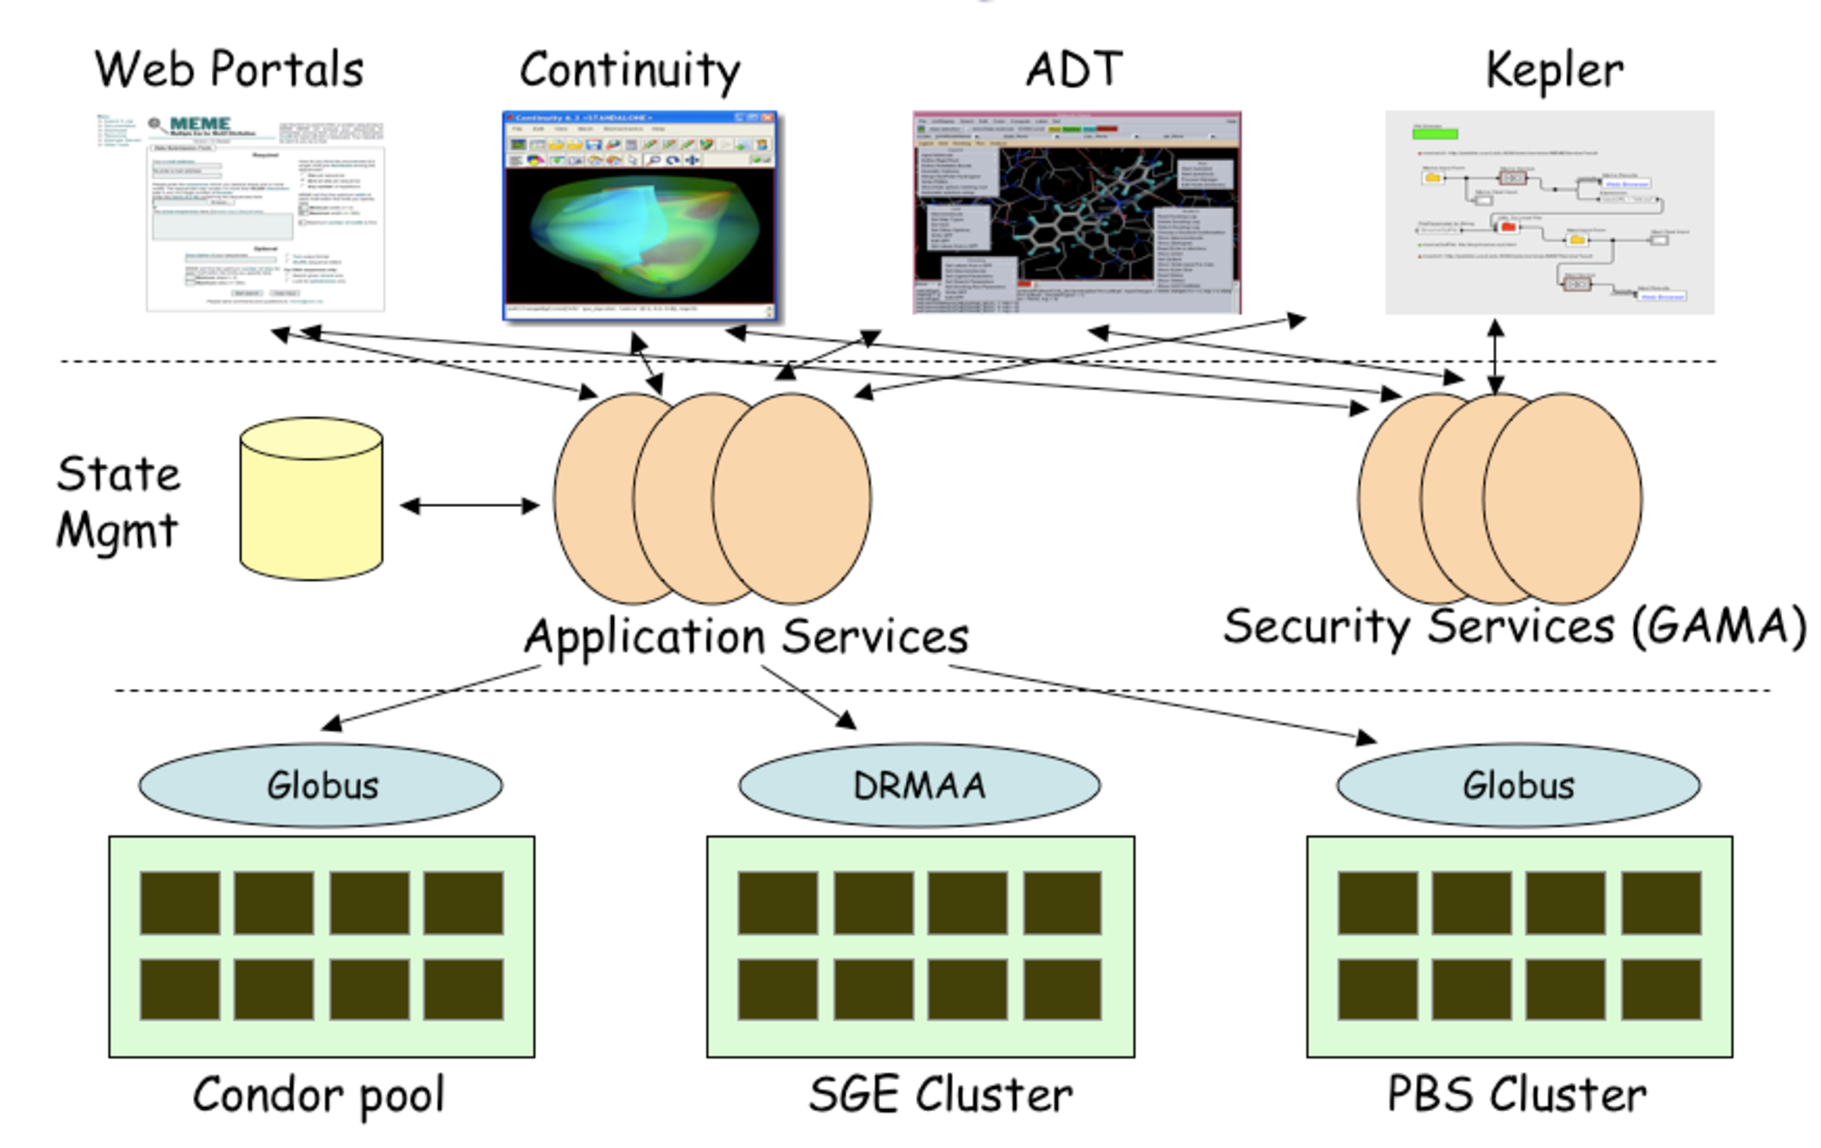
\includegraphics[width=8.5cm]{architecture}
\end{center}
\caption{Services Oriented Science using the Opal Toolkit}
\label{fig:arch}
\end{figure}

Although a detailed description of the Opal toolkit is beyond the scope of
this paper (and can be found in \cite{opal}), the overall architecture of
is shown in Figure \ref{fig:arch}. The salient features of Opal are as
follows:

\begin{enumerate}
\item{{\bf Scheduling and Cluster Management:} Since different sites use
    different schedulers such as SGE \cite{sge}, Condor \cite{condor},
    etc., Opal provides a uniform way to access them via standard APIs such
    as Globus GRAM \cite{gram} and DRMAA \cite{drmaa}. The schedulers are
    simply specified using a properties file, and Opal configures itself
    appropriately to access the schedulers via the appropriate parameters.
    In addition, we are currently also able to submit jobs to the CSF4
    metascheduler \cite{csf4} using its WSRF API \cite{wsrf} as described
    in \cite{opal-gui}.}

\item{{\bf Data management and Persistence:} The Opal toolkit manages the
    job data for a particular run on behalf of the user. Every job is run
    in a separate workspace so that multiple jobs from different users can
    be run concurrently. Furthermore, information about job status and
    outputs is persisted in a database to provide fault-tolerance for the
    services.}

\item{{\bf Security:} Opal services can be configured to use
    transport-level GSI-based \cite{gsi} security so as to restrict access
    to only authorized users.}

\item{{\bf Standardized WSDL API:} All Opal use a standard WSDL so that
    they can accessed in a uniform manner by different clients. We choose
    not to generate application specific WSDLs to avoid regneration of
    client-side stubs and rewriting of clients for every application.}

\item{{\bf Argument Description and Dynamic Interface Generation:} Opal
    services can be optionally configured with an XML specification for the
    command-line arguments. This specification consists of a description
    for flags, tagged and untagged parameters, and grouping of arguments.
    Flags are not ordered and are usually represented with a character
    prefixed with a dash and they activate a functionality in the
    application (e.g. -verbose). Tagged Parameters are usually formed by a
    prefix and input value (e.g. -input <filename>) - they can appear in
    any order. Untagged parameters are not prefixed, and hence their order
    is relevant. The argument description is mainly useful for two purposes
    - for validation of command-line arguments passed to the application,
    and for automatic interface generation. A detailed description of the
    argument description, and automatic generation of Web forms from the
    description is provided in \cite{opal-gui}. A complete lifecycle of
    this process is shown in Figure \ref{fig:opal-gui}.}

\end{enumerate}

\begin{figure}
\begin{center}
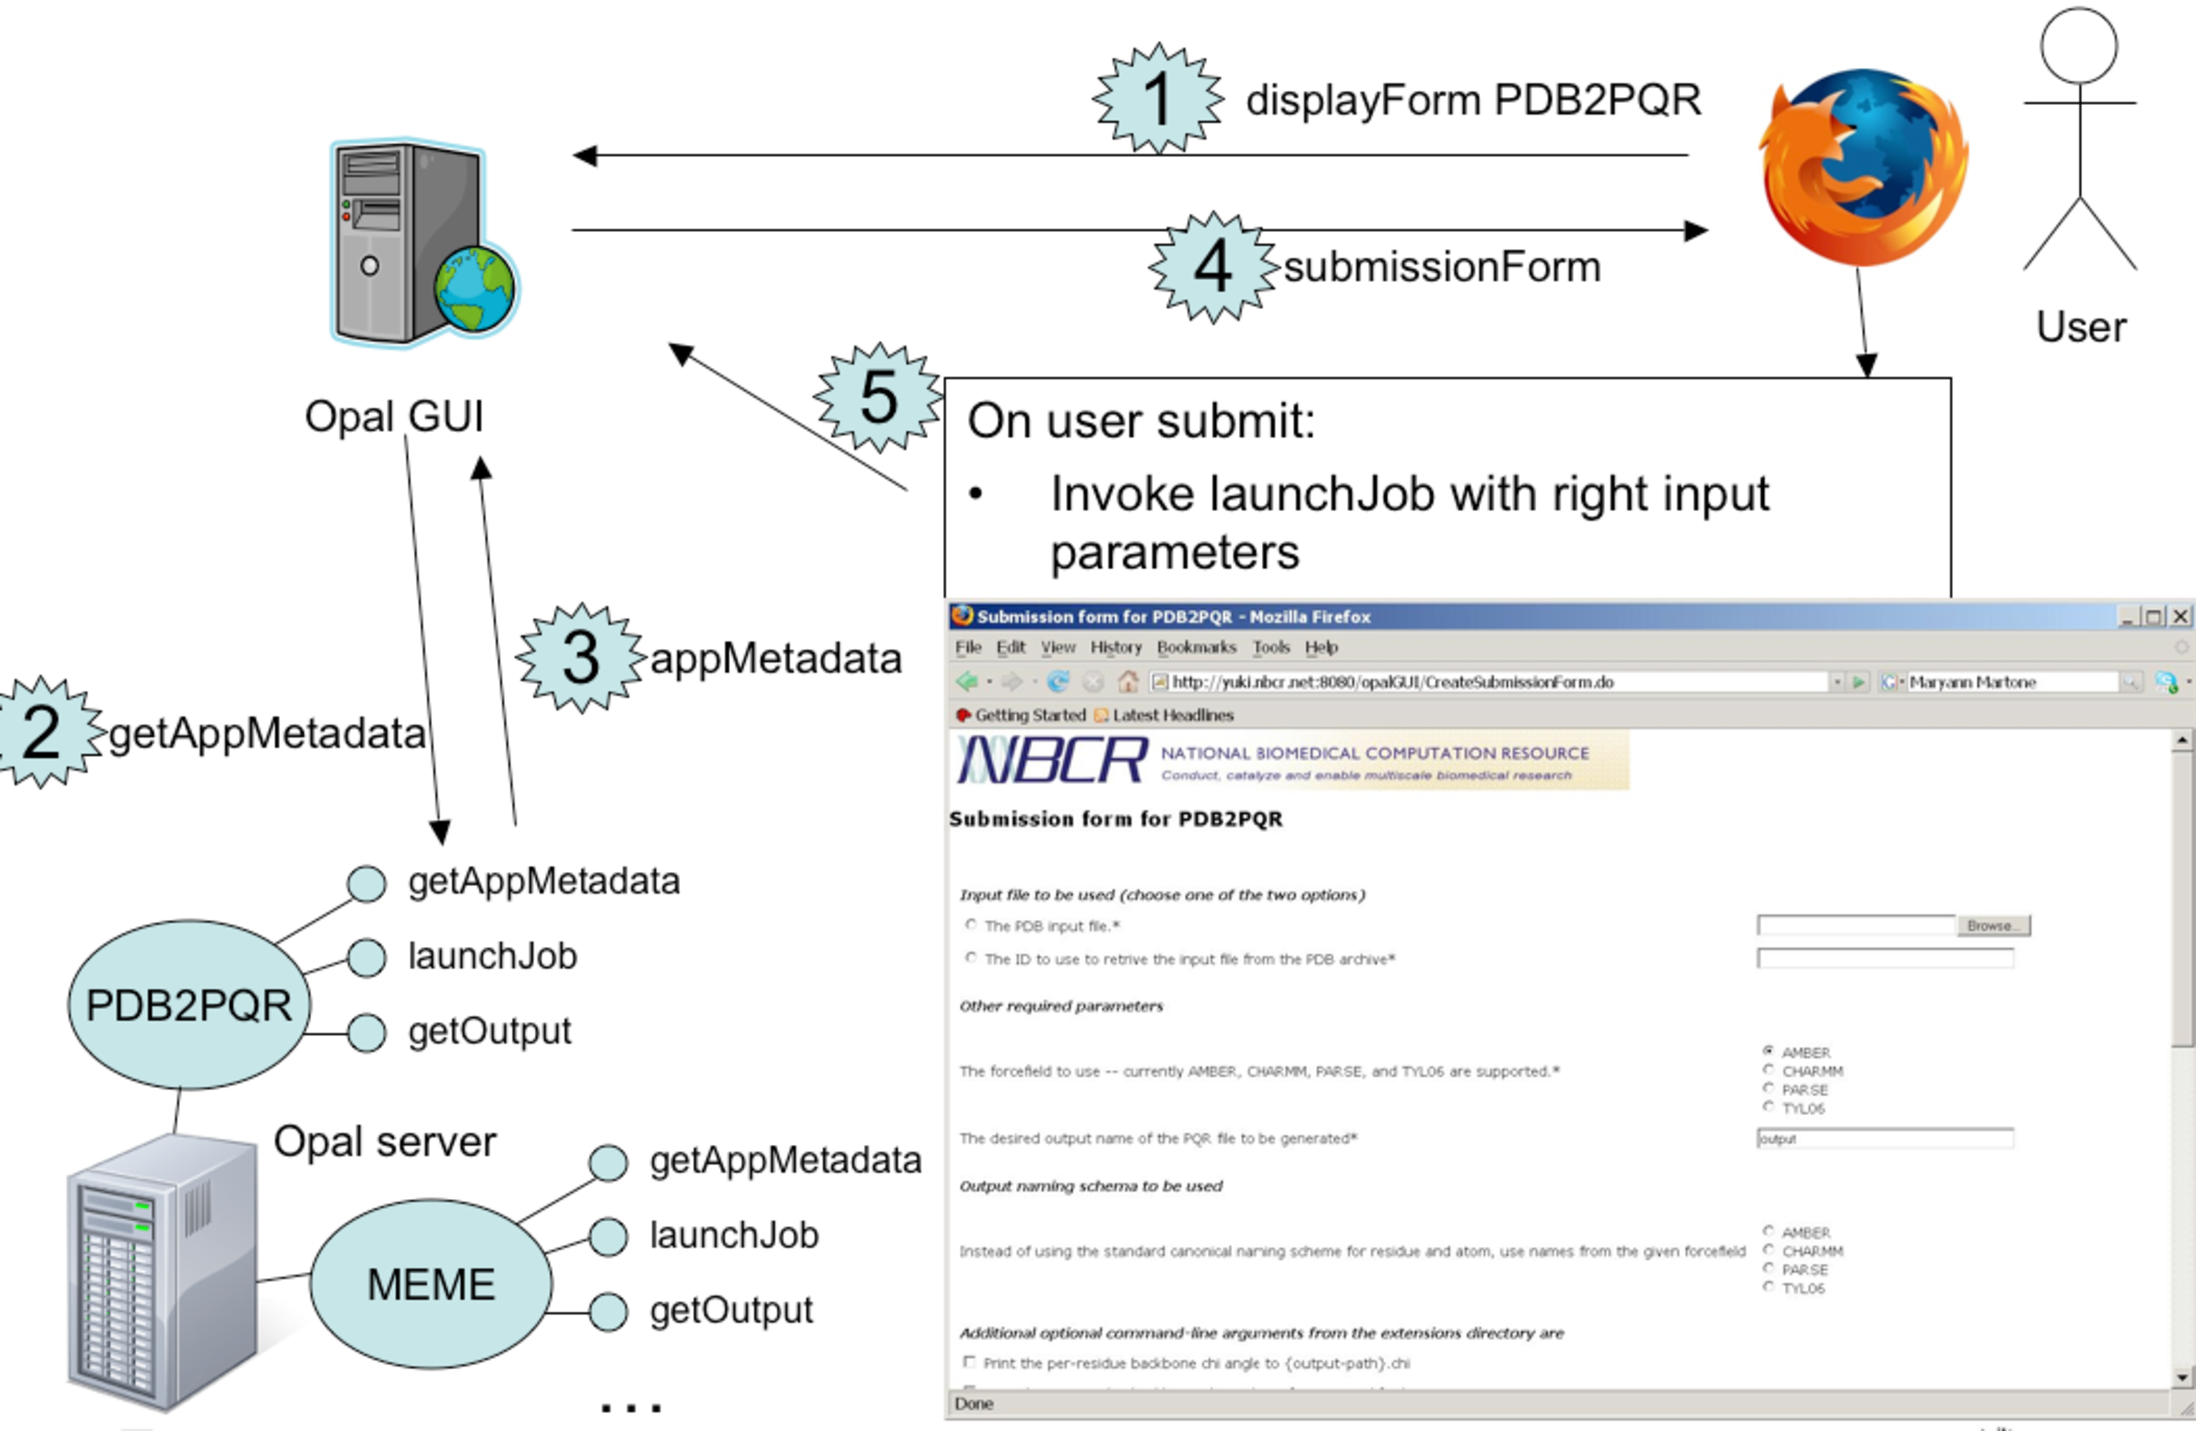
\includegraphics[width=8.5cm]{opal-gui}
\end{center}
\caption{Service Invocation via the Opal GUI}
\label{fig:opal-gui}
\end{figure}

The Opal toolkit is freely available from SourceForge, and uses an Open
Source BSD-style license. The current stable version of Opal at the time of
writing this manuscript is 1.9.3, and more information is available from
out website \cite{opal-website}.

- Towards Opal2

\begin{figure}
\begin{center}
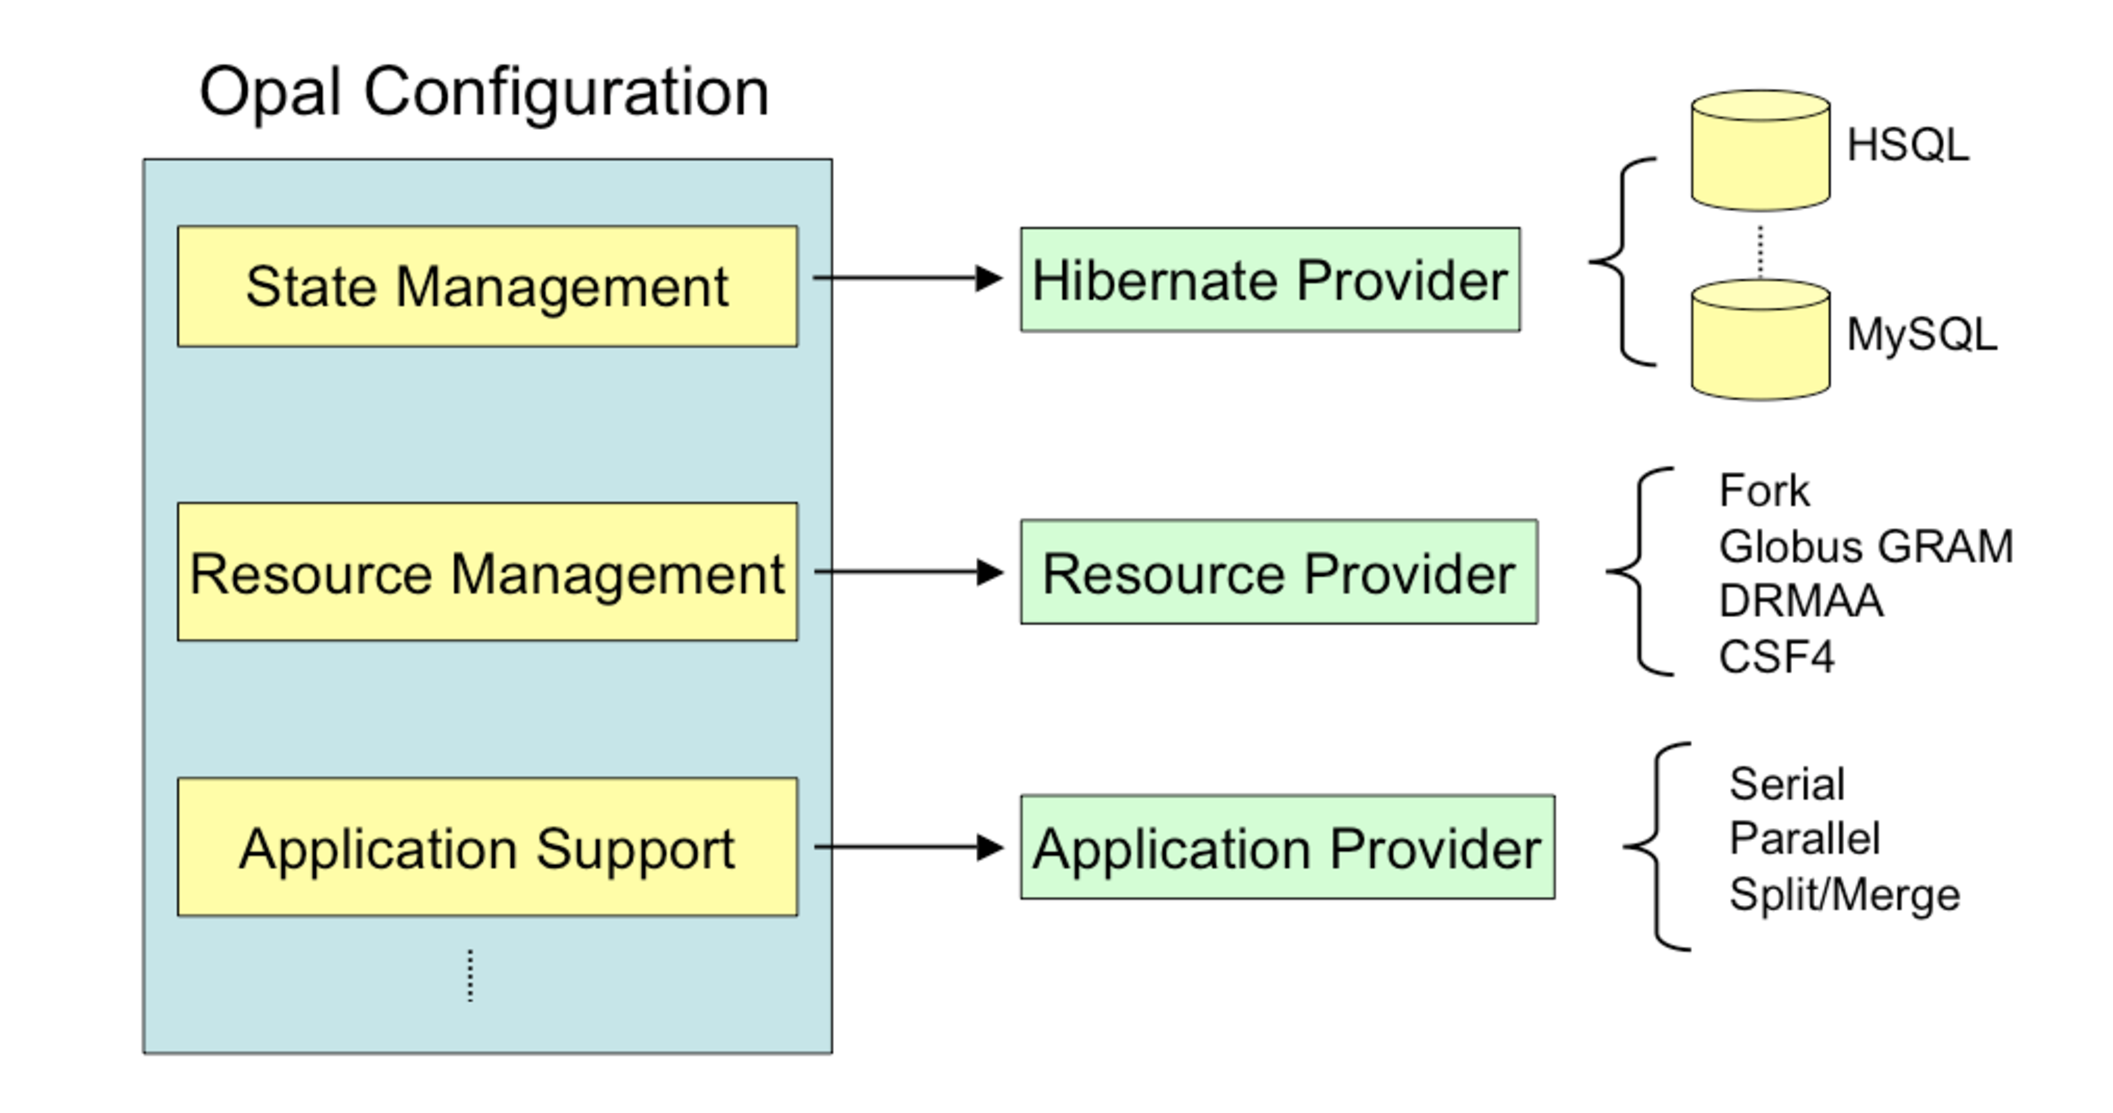
\includegraphics[width=9cm]{opal2-providers}
\end{center}
\caption{The Opal2 Provider Model}
\label{fig:opal2-providers}
\end{figure}

\section {Services-based Workflows in Vision}

- Vision based grid workflows (Michel, Guillaume, Sargis)

- Virtualization of Opal services (Sargis - something about how you
automatically create Vision nodes from the service list)

- Virtualization of Vision based workflows

  i) Use a local CLI opal client to access local or remote services (Sriram)

 ii) Automatic vision node creation through the opal client information
 service (Sriram, Guillaume - how the generated class is converted into a Vision node using introspection)

\begin{figure}
\begin{center}
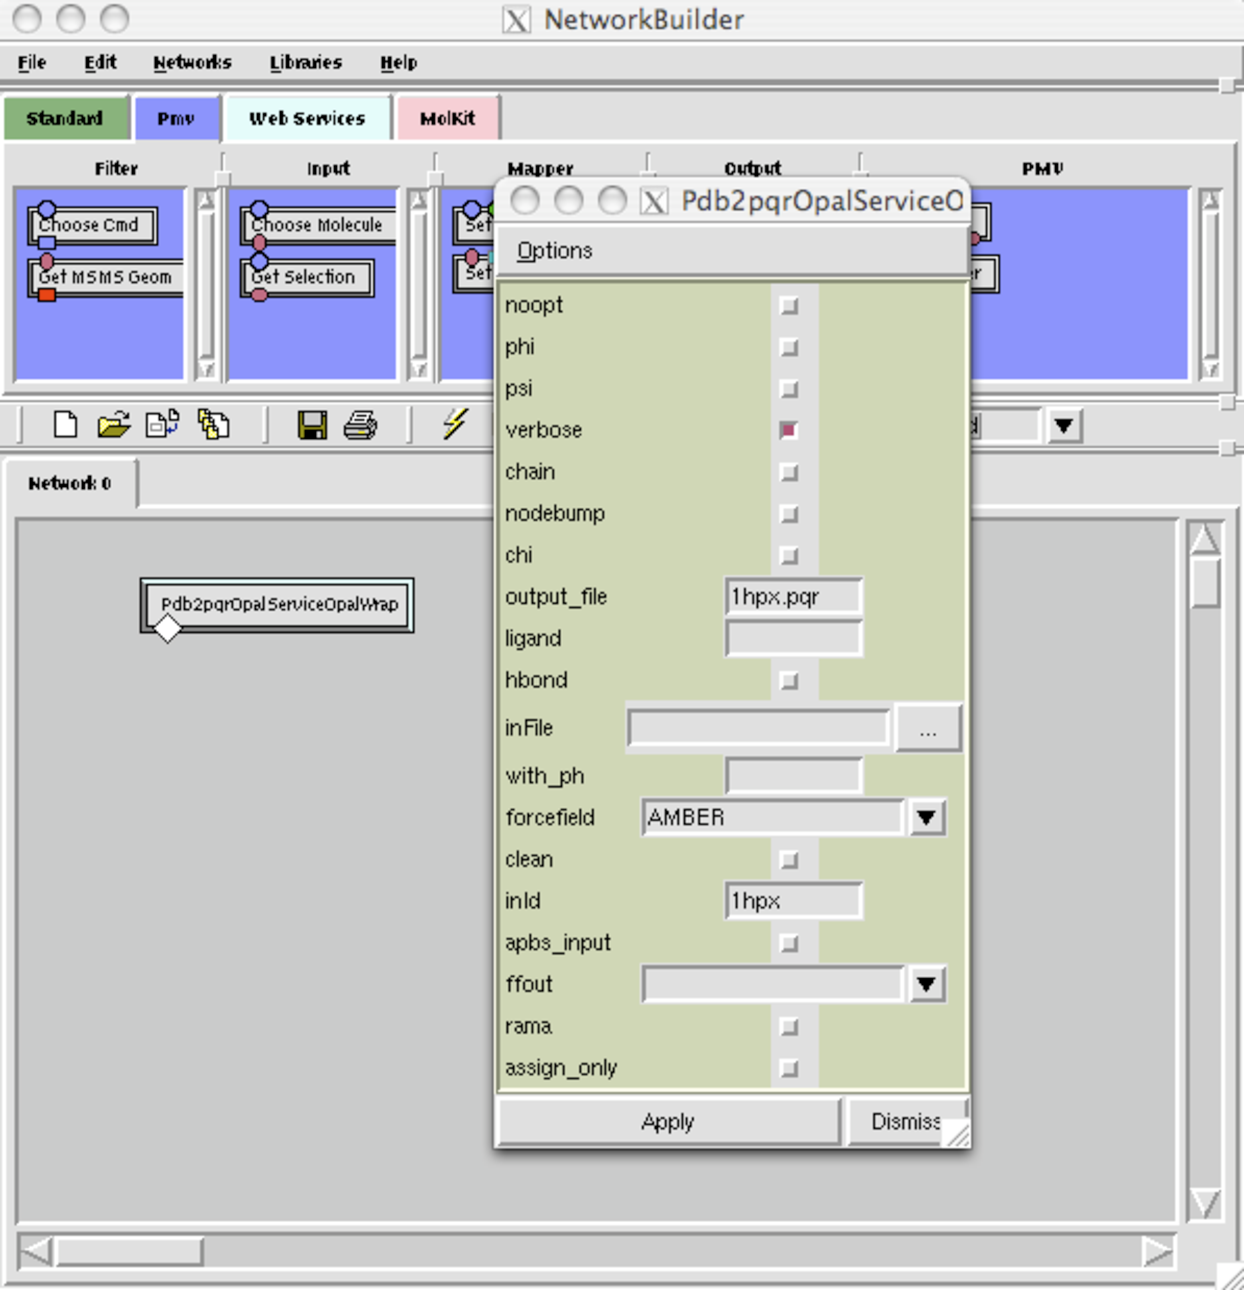
\includegraphics[width=8cm]{vision-gui}
\end{center}
\caption{Automatic interface generation for the PDB2PQR service in Vision}
\label{fig:vision-gui}
\end{figure}

- PDB2PQR-APBS workflow in action

% TODO: Need a more accurate screenshot
\begin{figure}
\begin{center}
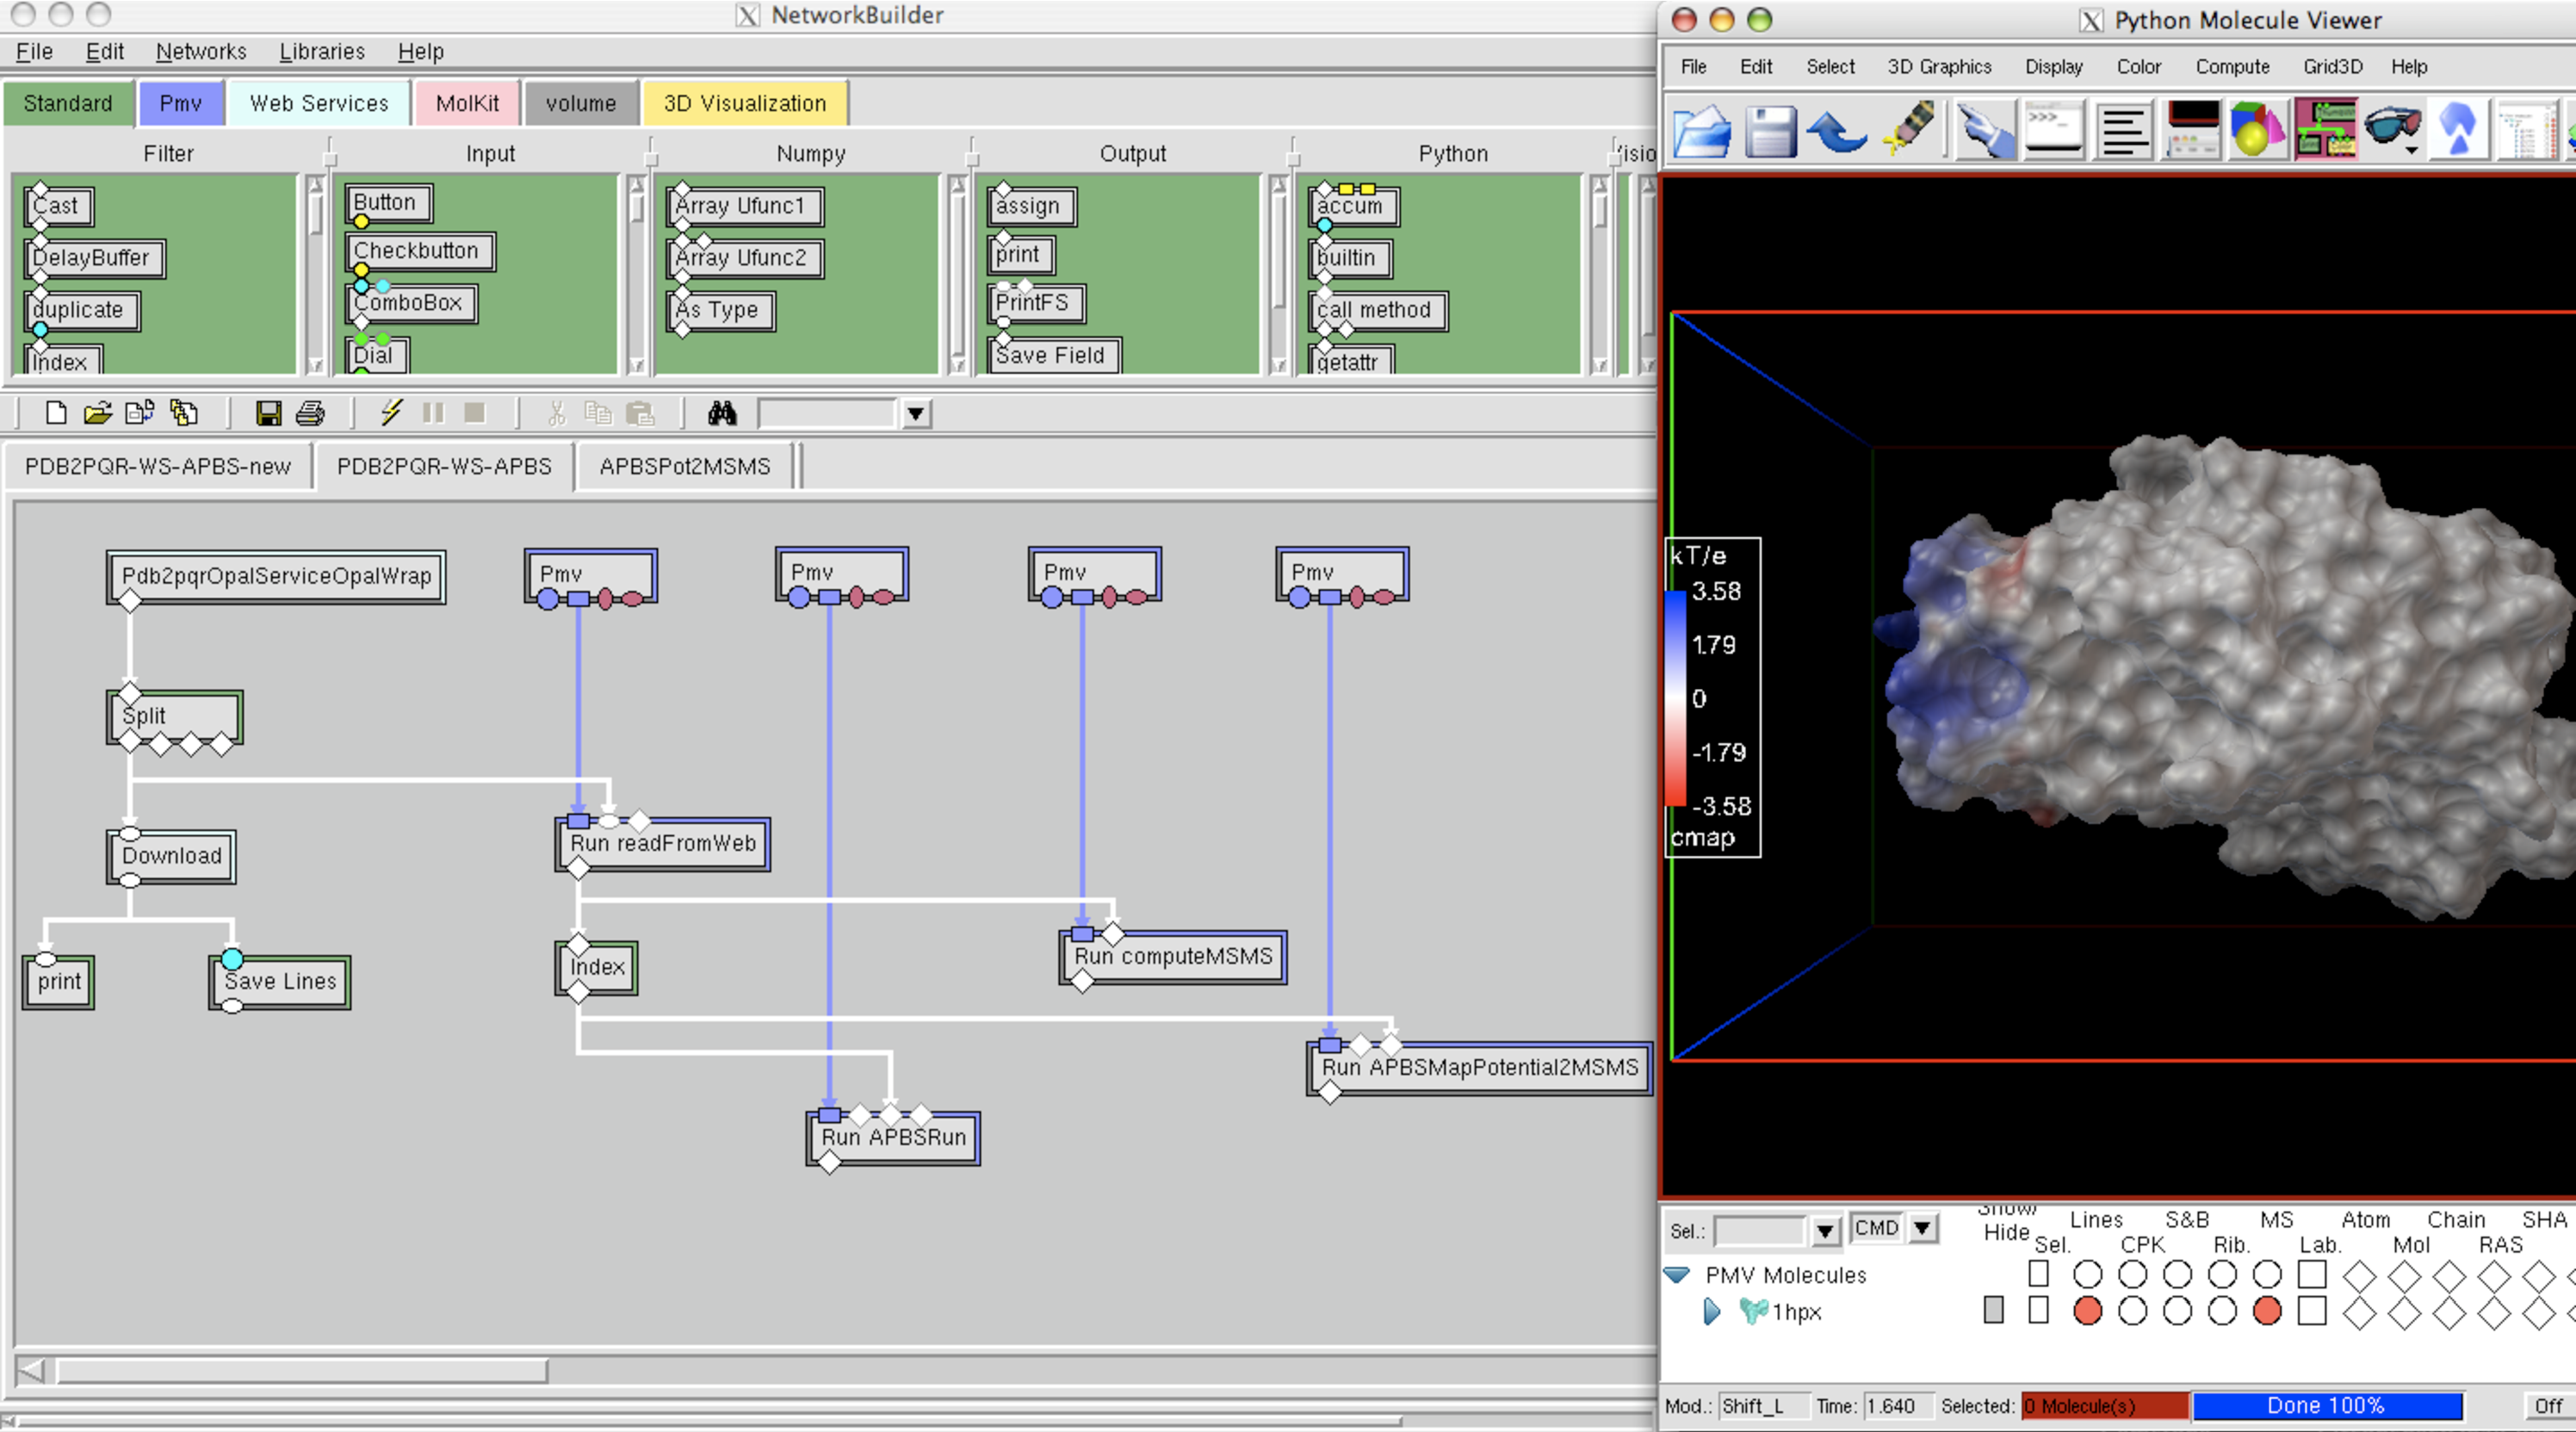
\includegraphics[width=8cm]{vision-workflow}
\end{center}
\caption{Vision worklow using local and remote services}
\label{fig:vision-workflow}
\end{figure}

\section {Discussion}

- How vision currently stores workflow (Michel)

- Fault tolerance (Michel, Sriram)

- Support for XPDL and other representations for workflows (Luca)

\section {Conclusions}

Visual programming environments enable non-programmers to intuitively and
interactively build scientific workflows and visualize their data, without
having to write code or understand the details of the back-end
infrastructure. In this paper, we described our tool called Vision, which
is a component-based, application-domain agnostic, cross-platform visual
programming environment. On the other hand, Grid computing provides an
enormous opportunity to scientific end-users to use distributed computing
and storage resources to enable novel science hitherto impossible using
traditional computing mechanisms. However, most Grid middleware tools are
complicated to install and too jargon rich for scientists to learn. In
order to simplify the use of Grid infrastructures, one has to provide easy
to use abstractions to the complex back-end functionality. Towards this
end, we have developed the Opal toolkit, which enables wrapping scientific
applications running on Grid resources as simple Web services, which can be
accessed via a number of user interfaces. In this paper, we described how
we can use the metadata provided by the Opal services to automatically
generate Vision nodes to access the applications running on Grid resources.
With the help of a molecular visualization workflow, we demonstrated how
this is being used by domain scientists, while being completely shielded
from the complexity of the back-end computational infrastructure. We
believe that the use of services-oriented science within visual programming
environments will go a long way towards lowering the entrance barrier for
scientific end-users to effectively use Grid middleware.

The authors would like to acknowledge support from the NIH P41 RR 08605 to
NBCR; TATRC W81XWH-07-2-0014 to PWA, the Gordon and Betty Moore Foundation
grant for the CAMERA project, and the NSF grants INT-0314015 and
OCI-0627026 for the PRAGMA project. 

%% References
\bibliographystyle{plain}
\bibliography{paper}

% that's all folks
\end{document}
